\newthought{Neuroscience as a whole} is concerned with the function of the nervous system. More precisely, it asks a very simple question: {\em What is the brain doing?}\footnote{ Or alternatively: {\em What is the nervous system doing?}} The simplicity with which humans and animals perform in their environment makes it almost unnatural to ask how their brains enable these behaviors. It is often hard to explain to laymen the complexity involved in preparing even the simplest actions, such as saccades or walking, such is the ease with which these are normally performed. One can not realistically expect to answer that question in any general fashion, I will however, try to touch upon a number of points which shed light on a number of aspects of the nervous system and provide us with a {\em guiding principle} to understand what the brain is doing and why and possibly how.\par
Neuroscience was born as a branch of biology, and although it is now often thought of as  an interdisciplinary science in itself, its objects of study are still to a large extent biological systems. Theodosius Dobzhansky published an influential essay in 1973, entitled {\em Nothing in biology makes sense except in the light of evolution}\cite{Dobzhansky1973}, which defends exactly that point. Though it has been reviewed and revisited constantly since its proposal, the theory of evolution through natural selection remains the central pillar of biological sciences. As such, neuroscience must also view its objects of study through the lenses of evolution. More specifically, we can then ask ourselves {\em What evolutionary advantage would this brain bring to an individual?} instead of {\em Why is the brain this way?} That being said,  there are caveats in the case of neuroscience. For one, the brain is capable of plasticity and adaptation unthinkable for other organs, and so we can not expect to understand the functionality of the brain in the same way which the shape of bird beaks can be understood as a function of their preferred fruits and seeds. Furthermore, the brain controls all of the motor and perceptual apparatus, having a multitude of uses and purposes, unlike simpler organs.\par
One particular aspect of the brain which has received increasing attention recently is its ability to deal with uncertainty. In a very productive line of research, a number of experiments have demonstrated that human and animal integrate uncertain information in a near-optimal way. The so-called {\em Bayesian Brain}\cite{Knill2004}, would explicitly represent the distribution over world states and perform inference in a manner consistent with Bayesian inference, obtaining optimal integration of sensory cues from different modalities, for example. It is still a matter of debate how these Bayesian computations would be implemented in the brain. One possibility is that the activity of neurons is sampling from a representation of the distribution of world states\cite{Berkes2011}, which is frequently called the {\em sampling hypothesis}. Another is that the activity of the neurons itself represents the likelihood over world states\cite{Ma2006}, and the population as a whole codes for the distribution, hence the term {\em population coding}.\par

\subsection*{Structure}
\newthought{The main goal of this thesis} is to develop a conceptual framework for studying optimal population coding in a dynamic framework. Furthermore, I would like to establish a link between optimal dynamic encoders and the efficient coding hypothesis, first proposed by Horace Barlow\cite{Barlow1961}. I believe that the inclusion of time into the coding framework raises a number of questions, which have not been addressed in the scientific literature properly. In the remainder of this chapter, I will discuss the efficient coding hypothesis and its more recent developments, and I will touch upon its relationship to Shannon's information theory\cite{Shannon1948}. I will finish by discussing the issue of dynamic population coding, highlighting the issues which I believe are of importance in considering the temporal aspect of coding. I will make the case for a study of optimal filtering of partially observed stimuli as a model of stimulus inference based on spike trains. Following, in \fref{chap:filtering}  I will introduce the general theory of filtering of stochastic stimuli. After that, in \fref{chap:MSE} I will discuss results regarding the Mean-Squared-Error (MSE) of optimal filters of point process data, presenting a number of new analytical results. In \fref{chap:control}, I will generalize the filtering framework to control problems, showing results for optimal control theory of point process-observed processes. In \fref{chap:optimal} I will then provide the connection to neuroscience, by considering the optimal encoding strategy for a population of neurons coding for a stochastic stimulus. I will then finalize by discussing the impact of the work presented and suggesting future research directions.\par

\subsection*{Contribution}
\newthought{The main contribution of this thesis} is in providing a conceptual toolbox to study optimal coding problems in a dynamic environment. I propose that the study of the average performance of an optimal Bayesian filter reconstructing the relevant stimulus provides a good measure of the quality of a dynamic code. Using this framework, I derive analytical results for the fast population code for dense populations of Gaussian neurons proposed by Quentin Huys\cite{Huys2007}. These are to my best knowledge the first results of this kind obtained for temporal coding of dynamic stimuli.

\section{Efficient Coding Hypothesis}

\newthought{The information} associated with a random event is defined as the logarithm of its inverse probability. This is at first nonintuitive, but with this definition, Shannon \cite{Shannon1948} has stated a number of interesting results regarding the coding and transmission of messages. We can further define the entropy of a distribution over a set of events as the average information conveyed by these events. So if we have a random variable $X$ taking values $x \in \mathcal{A}$ and a probability distribution $P : \mathcal{A} \to [0,1]$, we will have
$$
H(X)= \sum_x P_X(x) \log\left(\frac{1}{P_X(x)}\right).
$$
Furthermore, let us define the conditional entropy of two random variables as
$$
H(Y|X) = \sum_x P_X(x) \sum_y P_Y(y|x) \log\left(\frac{1}{P_Y(y|x)}\right),
$$
i.e. the conditional entropy is the average entropy of $Y$ given $X$, averaged over $X$. Let us also define the mutual information between $Y$ and $X$ as
$$
I(X;Y) = H(Y) - H(Y|X).
$$
Shannon regarded a noisy communication channel as a set of two random variables, one representing the message to be transmitted ($X$) and another representing the message received ($Y$). The noise in the channel would then be given by the conditional distribution of received messages given the transmitted messages ($P_Y(Y|X)$). The capacity of this channel is then given by
$$
C = \max_{P_X} I(X;Y).
$$
The rate of a given code is given by the number of bits needed to represent $X$ divided by the number of bits needed to represent $Y$, so if to send a one-bit message $x$ we must transmit a three-bit codeword $y$, our code would have a rate of $1/3$.
The noisy-channel coding theorem\cite{mackay2003information} then states
\begin{noisychannel}
\label{thm:noisychannel}
For every discrete memoryless channel with capacity $C$, for any $\epsilon>0$, any rate $R<C$, and for large enough $N$, there exists a code of length $N$ and rate $\leq R$ and a decoding algorithm such that the maximal probability of block error is $\epsilon$.
\end{noisychannel}
Before Shannon's work, it was generally believed that to achieve a vanishingly small error one would need a code with vanishingly small rate. The theorem shows, however, that one can achieve any rate below the channel capacity asymptotically.\par
Shannon's work had profound impacts throughout science. Horace Barlow proposed to use the redundancy of a code as a measure of its inefficiency. The redundancy of a code is given by
$$
\mathcal{R} = 1 - \frac{I(X;Y)}{C},
$$
and it quantifies how {\em efficiently} a given code encodes codewords $x$ into messages $y$. Note that in the case of a noiseless channel, this reduces to 
$$
\mathcal{R} = 1 - \frac{H(X)}{C}= 1 - \frac{H(Y)}{C}.
$$
The limit given by \fref{thm:noisychannel} then gives us the perfect redundancy-free channel. The {\em efficient coding hypothesis}, first proposed by Barlow\cite{Barlow1961} states that sensory relays in the nervous system recode the	messages to reduce the redundancy in them. Assuming that the transmission is noiseless we can then decompose the redundancy into two terms\cite{Atick1992}
$$
\mathcal{R} = \frac{1}{C} \left(C - \sum_i H(X_i) \right) + \frac{1}{C}\left(\sum_i H(X_i) -H(X)\right).
$$
The first term accounts for redundancy arising from unequal frequency of use of different symbols and the second accounts for redundancy arising from correlations between the symbols $X_i$. This can provide different approaches towards optimizing the coding mechanisms in the nervous system. In one popular example, Simon Laughlin related the distribution of contrasts in the natural environment of the blowfly to the tuning function of the large monopolar cells (LMC's) in the blowfly's visual system\cite{Laughlin1981}.


Since we are considering only one neuron, the analysis is somewhat simplified. Let us write the activity of the neuron as a function of the contrast $c$ as $o = g(c)$. We will then have that the redundancy of the firing is given by
$$
\mathcal{R} = \frac{1}{C} \left(C - H(O) \right),
$$
which is maximized when all output levels are equally probable. Further, we can say that
$$
P(o) do = P(c) dc, \textrm{ and therefore } o(c) = o_{max} \int_{-1}^c P(c') dc',
$$
as is shown in \fref{fig:laughlin}. This can be generalized to a number of cases, and Atick\cite{Atick1992} provided a thorough review of the framework. This approach is not, however, without its flaws.

\begin{marginfigure}
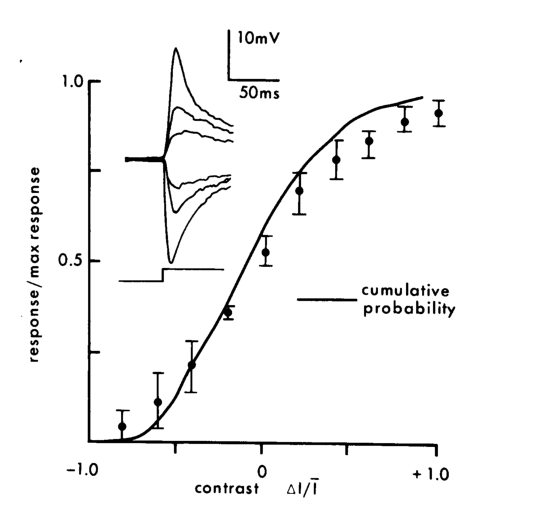
\includegraphics[width=\columnwidth]{figures/laughlin_81.eps}
\label{fig:laughlin}
\caption{The response function of the blowfly LMC closely resembles the cumulative distribution of visual contrasts in its natural environment. Figure taken from Laughlin, 1981}
\end{marginfigure}

\section{Dynamic Population Coding}


%The main goal of neuroscience is to answer a simple yet puzzling question: {\em What is the brain doing?} One might argue that we know a lot about what the brain is doing, at least on the phenomenological side, yet the more conceptual levels of what problem the brain is solving, or what it is good at doing, are far from answered. The main analogy we see in use in the field of neuroscience is that of the brain as a computer, hence the frequent use of concepts from Shannon's mathematical theory of communication. Namely, it is frequently hypothesized that the brain is optimally representing interesting aspects of the world it perceives. This thesis seeks to discuss the concept of optimal coding in neural systems. In it, I will discuss mainly findings in filtering of stochastic processes from point process observations and its relation to optimal population coding.\par
%Filtering is of general interest because of its relation to optimal control. More precisely, when considering a linear quadratic control problem under Gaussian noise conditions, the {\em separation principle} holds, and we can design an optimal controller by first predicting the state of the system, and then choosing the optimal control for the noiseless case on that state. The prediction step is solved by the Kalman filter. This framework is frequently used in the study of motor control, and a number of recent experiments and developments have relied on optimal control theory to model the properties of animal subjects under specific noise conditions. Here I will argue that the same approach should also be considered in the sensory areas of the brain.\par
%Investigators have repeatedly hypothesized that the shape of receptive fields and the response properties of sensory neurons can be traced back to optimality with respect to some criterion. The first approach, which drew heavily from Shannon's information theory, was Barlow's efficient coding hypothesis. In its initial form, it stated that the code employed in sensory systems should be adapted to the stimulus distribution in a way to minimized the redundancy, as defined in information theory as the difference between the code capacity and the source entropy divided by the code capacity. Many different efficiency measures have since been proposed. Metabolical considerations favor the use of sparse codes, where at any given time only a few neurons are active.\par
%Another popular approach is to use the Cramer-Rao bound of statistics, and maximize the fisher information of the code, so minimizing a lower bound on the mean-squared-error of the estimator. This has been very popular and is still widely employed in the theoretical neuroscience literature. This bound, however, has been proven to not be tight in useful regimes, and more recently a shift towards using the minimum of the mean-squared-error directly as an efficiency measure has been taking place. We focus here on this measure of efficiency, which we will motivate through optimal control theory in chapter ?? (INSERT REFERENCE).\par
%An alternative approach, which is still in its budding phase, is to consider directly optimal control problems and from the average cost incurred by a given code, choose an optimal code for a given task. This is hindered by the considerable analytical problems involved in treating optimal control problems analytically. I will show, however, that in the popular framework of dense Gaussian tuning functions, an exact expression can be found for the optimal cost-to-go of a linear-quadratic-Gaussian control problem. This bypasses the somewhat abstract notion of an efficiency criterion to consider directly the costs of a given code to the animal using it. It does so at the considerable expense of oversimplifying the problems faced by an animal to an impressive amount. Yet, the approach considers the problem of optimal coding from a more holistic perspective, considering representation and coding as a cog in a machine rather than and end in itself.\par
%
%\section{Structure}
%
%I will start out by reviewing the literature and the different approaches to optimal population coding in chapter ??, giving special attention to the case of mean-squared-error minimization which is considered in this thesis. In the following chapter, I briefly introduce the theory of filtering of point-process observed stochastic processes. Here, the general theory of filtering is presented and the simplifications introduced by the dense Gaussian tuning function limit are discussed. In the following chapter, I discuss results on the mean-squared-error in filtering of Gaussian processes, providing analytical results and comparing it to simulations. The derivations are also compared with a replica-type approach which yields the same results. In the following chapter I consider the problem of optimal control using point-process observations. This is discussed briefly, and a derivation for the optimal cost-to-go is presented. Finally, I consider the implications of the approaches developed to a ecological theory of sensory processing. Namely, I consider the relationship between optimal tuning widths and firing rates with the timescales and correlation lengths in the processes. This is also done numerically for a number of cases that are analytically intractable. I finalize by discussing the presented research, its impact and relation to previous research and future directions of research.
%\cite{susemihl2011}

%We will argue that filtering of stochastic processes is a good proxy for the neural representation of stimuli in the brain.\par

%This presents a number of problems, which we will address in this thesis.